% Chapter 1
\chapter{Definición del problema u oportunidad} % Main chapter title
\label{sec:problema} % For referencing the chapter elsewhere, use

Este capítulo debe contener la exposición general del problema. Con respecto al problema se debe responder las siguientes preguntas:
\begin{itemize}
	\item	¿Cuál es el problema u oportunidad abordado por el proyecto? ¿Es posible cuantificarlo?
	\item	¿Cuáles son las causas de la existencia de este problema u oportunidad? Haga referencia a publicaciones y/u otros antecedentes que validen estas causas.
	\item Explique cómo la memoria ayudará a abordar este problema.
	
\end{itemize}

% Citas a libro \cite{ejemploLibro} o paper~\cite{ejemploPaper}. Usted puede agregar otros tipos como journal o techincal report
\newpage

Falabella Tecnología Corporativa (FTC) posee actualmente un sistema de recomendación basado en Filtrado Colaborativo Implícito (Factorización de Matrices) desarrollado en BigQuery ML (BQML). Este sistema presenta limitaciones significativas para el negocio: su simplicidad dificulta abordar la complejidad del comportamiento del cliente, ofrece un bajo nivel de personalización y, crucialmente, utiliza únicamente el identificador del cliente como dato de entrada. Esta implementación desaprovecha una gran cantidad de datos relevantes, como características demográficas, comportamientos históricos y segmentaciones internas, restringiendo la capacidad del sistema para generar recomendaciones que maximicen la efectividad de las campañas de marketing.

¿Cuál es el problema u oportunidad abordado por el proyecto?

La principal oportunidad de mejora, identificada en conjunto con FTC, radica en mitigar el problema del \enquote{cold-start} o \enquote{arranque en frío}. Este problema afecta a clientes nuevos de una determinada unidad de negocio; es decir, aquellos que no cuentan con un historial previo de interacciones en dicha unidad, pero que sí poseen datos relevantes en las demás unidades de negocio del grupo Falabella. De este modo, el proyecto aborda la oportunidad de desarrollar un sistema de recomendación basado en dominios cruzados (Cross Domain Recommender Systems - CDRS) que utilice y conecte los datos de las diferentes unidades de negocio del grupo.

¿Se puede cuantificar?

La limitación del sistema actual genera un costo de oportunidad cuantificable. Como se detalla en la Figura \ref{fig:Limitaciones_Sistema_Actual}, existe un \textit{pool} de clientes que compran en las distintas unidades de negocio del grupo Falabella, pero que se encuentran en situación de \enquote{cold-start} en alguna de ellas. Por ejemplo, existen $3,27$ millones de clientes del grupo que no son clientes de \textbf{Falabella Retail}, $3,96$ millones que no lo son en \textbf{Sodimac} y $5,97$ millones para \textbf{Tottus}. Sumando las oportunidades de las tres unidades de negocio, se identifica un desaprovechamiento de más de $13,2$ millones de potenciales relaciones cliente-unidad que no pueden ser aprovechadas por la falta de un sistema de dominios cruzados.

\begin{figure}[th]
	\centering
	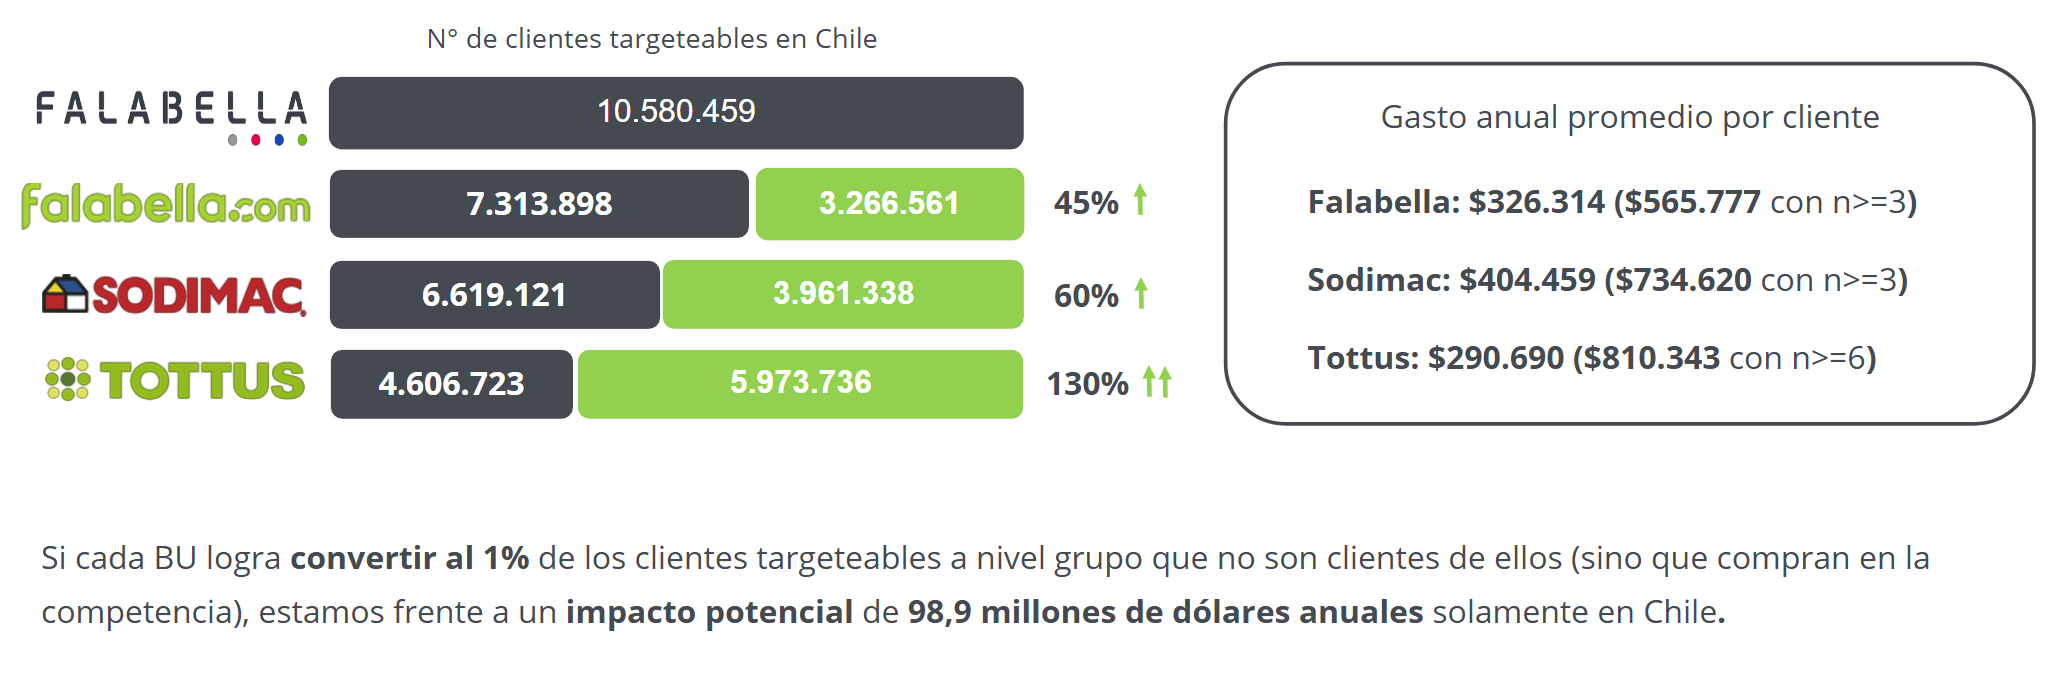
\includegraphics[width=\textwidth]{Figures/grafica Matias.png}
	\caption{Costo de oportunidad de las limitaciones del sistema de recomendación actual.}
	\label{fig:Limitaciones_Sistema_Actual}
\end{figure}

El impacto económico de esta oportunidad es significativo. Según estimaciones internas por parte de FTC, si cada unidad de negocio lograra convertir tan solo al $1\%$ de estos clientes \textit{targeteables} (utilizando los datos de dominios cruzados para mitigar el \enquote{cold-start}), se generaría un impacto potencial de aproximadamente $98,9$ millones de dólares anuales solo en Chile. Esta situación resalta la necesidad de mejorar el sistema de recomendación actual para maximizar los beneficios comerciales del grupo Falabella en un mercado altamente competitivo.


¿Cuáles son las causas de la existencia de de este problema u oportunidad?

Las causas de este problema son de naturaleza tanto técnica como estructural. En primer lugar, el sistema de recomendación actual es inherentemente limitado para escenarios de \enquote{cold-start}, ya que depende casi exclusivamente de interacciones pasadas %\cite{paper_sobre_limitaciones_MF}.
En segundo lugar, y de mayor relevancia para esta tesis, los datos de las distintas unidades de negocio del grupo Falabella no están integrados, de forma que la información de las interacciones de un cliente en \enquote{Falabella Retail} no se puede utilizar para apoyar las recomendaciones en \enquote{Sodimac}, pese a que el cliente es el mismo. Esta falta de una taxonomía unificada que conecte los catálogos de productos entre dominios es la causa principal que impide mitigar el \enquote{cold-start} mediante transferencia de información. %\cite{paper_sobre_cross_domain_RS}.

Explique cómo la memoria ayudará a abordar este problema.

En este contexto, la memoria de la tesis abordará el problema del \enquote{cold-start} en sistemas de recomendación mediante el desarrollo de un sistema basado en dominios cruzados (CDRS) que aproveche los datos de las diferentes unidades de negocio del grupo Falabella. El núcleo de esta propuesta consiste en la generación de \enquote{super-categorías} que vinculen productos entre las distintas unidades de negocio. Para ello, se diseñará un sistema de agentes de modelos de lenguaje grande (LLM) capaz de analizar, agrupar y etiquetar las categorías que sean similares para cada nivel (entiéndase los niveles de categorías como, por ejemplo, \enquote{categoría: Hombre, sub-categoría: Zapatos} para la unidad de negocio de Falabella Retail). Estos nuevos atributos (las \enquote{super-categorías}) se pueden utilizar como características adicionales en el sistema de recomendación, permitiendo realizar recomendaciones más personalizadas y precisas para clientes nuevos en situación de \enquote{cold-start} y, con ello, aumentar la probabilidad de que se conviertan en clientes recurrentes.